% ==================================================================
% ch04 -- from the research note "Engines and Individuals"
% ==================================================================
\chapter{Engines and Individuals}
\label{ch:eng}

\noindent
Composition assumed a common currency. Two learners sharing a wall were
drawing on the same tokens, and that assumption did a great deal of quiet
work. Drop it --- let each community's tokens be its own colour, as the
metabolisms of two separately originated biospheres would be --- and
something has to sit between them and convert.

That converter is this chapter's subject, and it turns out to be an organism
rather than a piece of infrastructure: a fourth access profile alongside
source and prey, persistent like a source, exhaustible like prey, and unique
in being adaptive in its \emph{rate}. It lives by the spread, which is not a
metaphor for a toll but literally the toll of the rendezvous through which
the swap happens. The nearest thing in the biosphere is not a decomposer but
a mycorrhizal network.

Two results give the chapter its title. The first is that the cycles of the
conversion graph form an error-correcting code, and that its total detecting
power is exactly the first Betti number of the graph --- so how much a
community can catch a mispriced exchange is a topological fact about the
shape of its trade, and a conversion sitting on a bridge can never be
checked at all. The second is a criterion for individuation. Communication
is not perfect; the notion is recovered by interposing a medium that may
drop or corrupt what passes through, and a region may close its namespace
exactly when the boundary it can maintain exceeds what the error rate costs.
An individual is where repair is cheaper than exposure. It is porous by
necessity --- perfect closure is death, for the same reason a solved science
is a dead ecology --- and it is a fixed point, since the closed region is
itself a learner that can compose with others.

That last move closes the loop the part opened with, and it is the natural
place to hand over. Once individuals are the sort of thing that can be
stacked, the question of what a learner sees from higher up in the stack is
no longer rhetorical --- which is where the next part begins.

\bigskip

%% ===================================================================
\section{Introduction}\label{eng:S1}

\subsection{Why the unit moves again}\label{eng:S1.1}

The series this note belongs to has moved its unit of analysis twice. In
\chSci the unit is a single mortal scientist: a cost-accounted
rho computation that forms hypotheses in a namespace logic, pays for its
assays, and dies when its stack runs out. In \chComp the unit is a
learner: a population of such computations together with their reservoirs,
serving as a namespace, with a distribution over it, composed with other
learners by parallel composition. That note ends by asking whether the
series individual/lineage/composite continues.

It does, and the reason it does is that composition of learners yields a
learner, so the construction is closed under an associative operator. But
closure alone gives arbitrary nesting and no scale structure: a soup of
composites has no distinguished levels. Something must pick out
\emph{skill}, \emph{organism}, \emph{pod}, \emph{species}, \emph{biosphere}
as rungs rather than as arbitrary cuts, and the companion notes do not say
what.

Two things were also missing from the economics. \chComp works in a
single token colour, so its conservation law is the flat statement that a
fixed supply $\Theta$ is never minted. Real coordination between
communities is not a transfer of one fungible fuel; it is
\emph{conversion}, at rates, between resources that are not interchangeable
--- and the arbitrage machinery of \cite{vtok} exists precisely to handle
that. And \chComp has no geometry: its composition operator is
indifferent to whether the two learners are adjacent or a galaxy apart,
though nothing in the framework says the cost of reaching across should be
the same in both cases.

This note supplies all three, and they turn out to be one thing.

\subsection{The move, stated once}\label{eng:S1.2}

Give each community its own token colour. Adjoin engines between colours
and weight each engine by its dissipation $\theta$. The resulting weighted
graph is the geometry the framework was missing; its cycle space is a code
on prices; and the isoperimetry of that graph is the criterion for when a
region may stop trading and start sharing --- that is, for when a
composition of learners becomes an individual.

\subsection{What we claim, and what we do not}\label{eng:S1.3}

We claim: that the engine is derivable as a fourth access profile rather
than importable as a new kind of thing (\S\ref{eng:sec:organism}); that
interposition supplies an error model natively, with $\theta$ as its
metering defect and stranding as its irreversibility
(\S\ref{eng:sec:medium}); that the
detection strength of a price is $1-\Reff$ and the total is $\bt$
(\S\ref{eng:sec:code}, Theorem~\ref{eng:thm:foster}); that inventory-holding
engines make arbitrage a property of a marking (\S\ref{eng:sec:fork}); that
merger is available exactly inside an isoperimetric threshold
(\S\ref{eng:sec:indiv}, Proposition~\ref{eng:prop:indiv}), with partial closure of
the medium namespace as its structural form
(Definition~\ref{eng:def:indiv}); and that a finite critical radius, together
with the tower of media, forces the hierarchy that \chComp could
only permit (\S\ref{eng:sec:hier}).

We do not claim to have derived the rates. \cite{vtok} takes them as given
and so, in the main, do we; \S\ref{eng:sec:rates} says what it would take to
derive them and why the numbers of \chGame are the natural candidate.
We do not claim the error channel has been identified: \S\ref{eng:sec:whicheps}
inherits, unresolved, the ``which $\varepsilon$ is binding'' question of
\cite{compaut}. We do not claim the correspondence with observed biology is
more than suggestive, though \S\ref{eng:sec:decay} notes that the ecological
pyramid falls out of Proposition~2 of \cite{vtok} with no adjustment, which
is a check we did not arrange.

%% ===================================================================
\section{What this chapter carries forward}\label{eng:S2}

From \chSci: the cut and the three grades of access (perception,
interaction, reflection); the assay via the \texttt{where} clause; the
conservation law $\sigma + \kappa = \sigma_0 = \Theta$; the access profile
distinguishing a \emph{source} (persistent emitter, rate-limited,
non-exclusive, non-adaptive) from \emph{prey} (linear send, exhaustible,
exclusive, adaptive); the relaxation lattice and its ultrametric; and the
freshness-by-quotation proposition, that for any context $C$ with
$C[P] \neq P$ the name $@C[P]$ does not occur in $P$.

From \chGame: the two routes to any predicate --- \emph{read} it,
priced by formula depth, if the environment has computed it into legible
structure, or \emph{drive} it, priced by rendezvous --- and the observation
that the interesting question is not whether the work is done but who is
billed for it.

From \chComp: the learner as three layers (population, namespace,
distribution) with the distribution \emph{inside}; composition as parallel
composition; the factorisation theorem, that namespace disjointness is
equivalent to absence of a spanning redex and to $\mu_{12} =
\mu_1 \otimes \mu_2$; the grading vector
$\mathbf{k} = (k_{\mathrm{met}}, k_{\mathrm{src}}, k_{\mathrm{prb}},
k_{\mathrm{mat}})$ over the four typed namespaces $\Met, \Src, \Prb, \Mat$;
merger $\Merge$ as a separate operator; the instability of non-interference
and its repair by rooting; and competitive dilution in closed form.

From \cite{CARho} and \cite{CE}: signatures as names, token stacks as
first-class terms, wrapping by construction, the cost monad
$(\mathrm{Cost}, \eta, \mu)$ on $\mathrm{ciGSLT}$ and its non-idempotence,
and located resource stacks.

From \cite{finrho}: the correction that a stack floating in the
associative--commutative soup is ambient authority, repaired by holding
every stack on a channel; the acceptance gate; the netting result; and the
four cost-accounting patterns.

From \cite{vtok}: conversion systems, engines, rates with
$r(a{\to}b)\,r(b{\to}a) = 1$; the log-rate cochain $\ell$; the equivalence
of arbitrage-freedom, exactness of $\ell$, and existence of a valuation
$\nu$; the graph--Hodge splitting into energy and arbitrage components;
$\dim\ker\delta^\ast = \bt$; arbitrage-removal as an idempotent reflection;
the first law (conservation of $\nu$ in the lossless regime); the second
(dissipation $\theta$ makes $\nu$ a Lyapunov function); and the insistence
that $\nu$ is a unit of account and never a medium of exchange.

From \cite{compaut}: the crossover between a shared substrate and
autonomous replication, at critical radius $r^\ast \sim
\sqrt{\rho v / \varepsilon}$ in an error rate $\varepsilon$, a repair
throughput $\rho$, and a communication speed $v$; and the closing
conjecture that this crossover and the factoring of the OSLF-generated
logic over a population are two views of one threshold. That conjecture is
what \S\ref{eng:sec:indiv} cashes.

From \cite{KnotsNote}: the persistent boundary-forwarder lemma, which is what
makes an encoding compositional and which supplies
Proposition~\ref{eng:prop:wlog}; and the diagnosis, made there, that a
mediating process written with a linear receipt models one passage rather
than a passage-way.

From \cite{SPJ2000}: the combinators \texttt{zero}, \texttt{one},
\texttt{give}, \texttt{and}, \texttt{or}, \texttt{scale},
\texttt{truncate}, \texttt{get}, and observables.

%% ===================================================================
\section{Colours, engines, and a fork in the conservation law}\label{eng:S3}
\label{eng:sec:fork}

\subsection{Communities are colours}\label{eng:S3.1}

\begin{definition}[Coloured learner]\label{eng:coloured-learner}
A \emph{coloured learner} is a learner $\Lrn$ in the sense of
\S\ref{com:S3} of \chComp together with a distinguished signature
$c(\Lrn) \in \Sig$, its \emph{colour}: the signature at the head of every
stack held at a name in $\Met(\Lrn)$.
\end{definition}

The colour is not new apparatus. \cite{CARho} already replaces one
universal fuel by a family of signature-indexed resources, one per
economically empowered actor; \cite[\S6]{CARho} calls the collapse to a
single $s_0$ the monochromatic limit. \chComp works in that limit.
Taking a community's colour to be its own signature is the natural
un-collapsing, and it is what makes ``Terran food and alt-Earth food may
not be mutually nutritive'' a statement the calculus can express: two
learners whose $\Met$ stacks carry incomparable signatures cannot eat each
other's tokens, however adjacent they are.

\begin{definition}[Engine]\label{eng:def:engine}
An \emph{engine} between colours $a$ and $b$ is a persistent process
holding two located reserves, one of each colour, and offering a linear
swap: it accepts one $a$-token and releases $r(a{\to}b)$ $b$-tokens from
its own inventory. Its \emph{toll} is the metering charge of the rendezvous
that performs the swap.
\end{definition}

\subsection{The fork}\label{eng:S3.2}

There is a conservation collision here that must be settled before
anything else, because the two notes being joined conserve different
things. \chComp conserves tokens \emph{per colour}: $\Theta$ is
fixed and never minted. \cite{vtok} conserves the scalar $\nu$: an engine
consumes one $a$ and releases $r$ units of $b$, which is not per-colour
conserving at all. One must give.

\begin{itemize}[itemsep=3pt]
\item[(i)] \textbf{Engines hold inventory.} A swap is against stock, so
per-colour totals \emph{are} conserved and $r$ is the ratio at which
inventory is exchanged. The cost: engines deplete, $r$ moves with the
marking, and $\ell$ becomes a function of state.
\item[(ii)] \textbf{Conserve only $\nu$.} Colours interconvert at fixed
rates and $\Theta_\nu$ is the invariant. This matches \cite{vtok} exactly
but abandons the per-signature ledger the scientist note runs on.
\end{itemize}

We take (i). It preserves the more specific law, it keeps engines mortal
(an engine that runs out of one colour stops being an engine, which is what
we want of an organism), and its cost --- state-dependence --- is where the
content is.

\begin{proposition}[Arbitrage is a property of a marking]\label{eng:prop:marking}
Under (i) the log-rate cochain is a function $\ell(M)$ of the marking $M$
of the engine reserves. Consequently the Hodge splitting
$\ell = \ell_{\mathrm{en}} + \ell_{\mathrm{arb}}$ of \cite[\S4]{vtok} must
be taken pointwise in $M$, and arbitrage-freedom is a condition on a
\emph{state} of the ecology rather than on the ecology.
\end{proposition}

\begin{proof}
Immediate from Definition~\ref{eng:def:engine}: the rate is computed from the
reserves, and a swap changes the reserves. Appendix~\ref{eng:app:repro},
block~(4), exhibits a triangle of constant-product engines whose cycle
yield is exactly $1$ at the balanced marking and departs monotonically as
one engine is drained; six trades of ten units carry
$\log \oint \ell$ from $0$ to $-1.003$.
\end{proof}

\begin{remark}[Trading is what removes arbitrage]\label{eng:trading-what-removes-arbitrage}
Proposition~\ref{eng:prop:marking} is not a defect. In \cite{vtok} the
projection $\Pi$ onto the exact cochains is a least-squares correction
performed by nobody in particular; the note flags that the operational
content of ``shaking the arbitrage out'' is left abstract. Under (i) it is
concrete and it is metabolic: an arbitrageur is a computation that traces a
cycle of yield $> 1$, and each pass moves the reserves in the direction
that reduces the yield. Arbitrage-removal is not applied to the system, it
is \emph{eaten out} of the system, and the eating is metered like anything
else. This is the sense in which the idempotent reflection of
\cite[Prop.~3.4]{vtok} is realised rather than postulated.
\end{remark}

\begin{corollary}[Residual arbitrage]\label{eng:cor:residual}
Since each pass of a cycle costs the arbitrageur at least one token, and
the yield per pass falls monotonically toward $1$, there is a level of
arbitrage below which removal is unprofitable. A mortal ecology therefore
carries a floor of arbitrage set by its own metering, and the floor is
higher the poorer the ecology.
\end{corollary}

Corollary~\ref{eng:cor:residual} is \chSci, Corollary~\ref{sci:cor:poverty} --- poverty is
confining --- one level up and in a second currency. A rich ecology has
efficient prices for the same reason a rich scientist can afford deep
inquiry.

\subsection{The reflexive observable}\label{eng:S3.3}

In \cite{SPJ2000} an observable is a time-varying quantity both parties
agree on, and it is exogenous: the weather, a stock price, a block height.
Under (i) the observable that sets an engine's rate reads the engine's own
inventory. This is the one place the combinator language had to be
extended, and it is worth naming, because it is what turns a contract into
an organism: the contract's terms depend on the contract's state.

%% ===================================================================
\section{The engine is an organism}\label{eng:S4}
\label{eng:sec:organism}

\subsection{A fourth access profile}\label{eng:S4.1}

\S\ref{sci:S10} of \chSci separates two ways of being food. A \emph{source} is
a persistent emitter: rate-limited, non-exclusive, non-adaptive,
inexhaustible on the timescale of one learner though finite in the
aggregate. \emph{Prey} is a linear send: exhaustible, exclusive, adaptive.
The distinction is not a distinction of sort or of rewrite rule but of
multiplicity --- a fact about the cut.

The engine is a third way, and it is obtained by taking the same four
attributes and choosing a combination the table did not previously contain.

\begin{table}[t]
\centering\small
\fitwidth{%
\begin{tabular}{@{}lcccc@{}}
\toprule
& \textbf{persistent} & \textbf{exclusive} & \textbf{exhaustible}
& \textbf{adaptive} \\
\midrule
Source          & yes & no  & in aggregate & no \\
Prey            & no  & yes & yes          & yes \\
Scientist       & ---as prey, plus grade-3 exposure--- & & & \\
\textbf{Engine} & \textbf{yes} & \textbf{no} & \textbf{per colour}
                & \textbf{in rate} \\
\bottomrule
\end{tabular}}
\caption{The engine as a fourth access profile. It is source-like in
persistence and non-exclusivity, prey-like in exhaustibility, and unique
in that what adapts is not its behaviour under attack but its
\emph{terms}.}
\label{eng:tab:profiles}
\end{table}

\begin{proposition}[The engine is derived, not imported]\label{eng:engine-derived-imported}
The profile in Table~\ref{eng:tab:profiles} requires no new sort, no new
rewrite rule, and no new GSLT. A persistent receipt on a quote channel
supplies persistence and non-exclusivity; two located reserves supply
per-colour exhaustibility; and computing the rate from those reserves
supplies rate-adaptivity. All three are available in the host calculus of
\chSci.
\end{proposition}

\begin{proof}
Appendix~\ref{eng:app:rho} exhibits the term. Persistence is \texttt{<=};
location is a channel, per \cite[\S2.2]{finrho}; the rate is a
\texttt{for}-comprehension over the reserve channels that replaces what it
reads.
\end{proof}

\begin{remark}[The persistence is load-bearing]\label{eng:persistence-load-bearing}
An engine written with a linear receipt models one conversion, not a
converter --- the same bug found and fixed in the knot encoding, where
crossing gates written with \texttt{<-} evaporate after a single
visitation and model one passage through the diagram rather than the
diagram. The correct shape is a \emph{persistent issuer} offering
\emph{linear} contracts: the enzyme persists, the substrate binding does
not.
\end{remark}

\begin{remark}[What the engine eats]\label{eng:rem:eats}
\cite[\S6]{vtok} introduces dissipation $\theta(a{\to}b) \geq 0$ as a
modelling parameter and reads the resulting inequality as the second law.
Here $\theta$ is not posited. Every rendezvous is metered, and the swap is
a rendezvous, so $\theta$ \emph{is} the toll --- and it accrues to the
engine's own stack, because something has to fund the engine's continued
existence and nothing else is available. The second law and the engine's
metabolism are the same fact. An engine whose traffic falls below its burn
rate starves, exactly as a scientist does.
\end{remark}

\begin{remark}[Not a decomposer]\label{eng:decomposer}
It is tempting to call the engine a decomposer, on the grounds that it
lives on what others cannot metabolise. The better analogue is the
mycorrhizal network \cite{kiers}: it does not consume waste, it makes two
otherwise incommensurable metabolisms mutually available and takes a cut.
That literature is also the right prior art for
\S\ref{eng:sec:bridge}, since it studies exchange rates set by partner choice
and outside options rather than by no-arbitrage \cite{noe}.
\end{remark}

\subsection{The combinators as reaction language}\label{eng:S4.2}

With the organism identified, the combinators of \cite{SPJ2000} sit one
level down: they name the engine's reactions, not the engine.

\texttt{one}$(k)$ is the funded unit transfer; \texttt{give} swaps which
signature funds the leg, which \cite[\S3.1]{finrho} observes is exactly the
two-sided surface of the cut made operational. \texttt{scale}$(o,c)$
carries the rate, and by \cite[\S3.6]{finrho} scaling multiplies the amount
moved and \emph{not} the fuel demand --- cost counts funded rendezvous, not
magnitude. \texttt{and} is the atomic join, under which the partial-funding
hazard is structurally impossible.

\begin{observation}[The swap is the netted futures shape]\label{eng:swap-netted-futures-shape}
An engine's conversion is
\[
  \texttt{and}\bigl(\texttt{scale}(o,\texttt{one}(a)),\;
                    \texttt{give}(\texttt{one}(b))\bigr),
\]
Pattern~(A) of \cite[Tab.~1]{finrho}, bilateral cash settlement. That
note shows the apparatus rewards the netted form: one transfer in the
data-dependent direction instead of two gross legs, atomic by construction
and costing one token instead of two.
\end{observation}

\begin{corollary}[Netting is thermodynamic]\label{eng:netting-thermodynamic}
Since $\theta$ is the toll (Remark~\ref{eng:rem:eats}), netting halves the
dissipation on every conversion. What \cite{finrho} presents as a
settlement optimisation is, in this reading, a reduction of the second-law
loss along every edge of the engine graph, and hence --- by
\S\ref{eng:sec:decay} --- an increase in the profitable radius.
\end{corollary}

The temporal combinators do work too, and \S\ref{eng:sec:credit} takes them up.

%% ===================================================================
\section{The medium}\label{eng:S5}
\label{eng:sec:medium}

\subsection{Interposition is without loss of generality}\label{eng:S5.1}

The host calculus takes communication to be perfect. It does so without
loss of generality, because imperfection can be modelled as an additional
process rather than an additional rule: races and higher-order channels
suffice. Generalise
\[
  \texttt{for}(y \leftarrow x)P \mid x!(Q)
  \qquad\text{to}\qquad
  \texttt{for}(y \leftarrow x_1)P \mid C(x_1,x_2) \mid x_2!(Q),
\]
where $C$ is any process joining the two endpoints. The simplest $C$ is a
persistent two-way forwarder; richer ones do arbitrarily more.

\begin{proposition}[The perfect case is a special case]\label{eng:prop:wlog}
When $C$ is the persistent two-way forwarder on $(x_1,x_2)$, the interposed
term is weakly bisimilar to the direct one. Hence nothing is lost by
working in the general form, and the perfect-communication calculus is
recovered as the identity medium.
\end{proposition}

\begin{proof}[Proof sketch]
This is the boundary-forwarder lemma of the knot encoding
\cite{KnotsNote}, whose persistence is exactly what makes the encoding
compositional. The forwarding steps are $\tau$ and are absorbed by weak
bisimulation; persistence is required, since a linear forwarder relays once
and then is not a channel.
\end{proof}

\begin{definition}[Loss and corruption]\label{eng:loss-corruption}
A medium \emph{drops} when it receives on $x_1$ and emits nothing, and
\emph{corrupts} when it emits a value other than the one received. Write
$p \in (0,1]$ for the per-hop probability that a message is relayed
faithfully.
\end{definition}

\begin{remark}[Interposition is not cost-preserving, and that is $\theta$]
\label{eng:rem:notmorphism}
Proposition~\ref{eng:prop:wlog} is a statement about behaviour, not about
metering: a single gated rendezvous becomes at least two. So interposition
is not a morphism in the cost-accounted category of \cite{CE} --- it
multiplies the gated transitions rather than preserving them --- and the
defect is exactly the dissipation $\theta$ that \S\ref{eng:sec:organism}
attributes to the engine. This is the third instance in the series of one
pattern: in \S\ref{com:S4.3} of \chComp the lax comparison map's defect is the
interaction; here the interposition's defect is the cost of distance.
Distance is not a parameter of this calculus. Distance is interposition,
and its price is the failure of a map to be strict.
\end{remark}

\subsection{A ladder of media}\label{eng:S5.2}

\begin{table}[t]
\centering\small
\fitwidth{%
\begin{tabular}{@{}lll@{}}
\toprule
\textbf{Rung} & \textbf{What $C$ does} & \textbf{What it contributes} \\
\midrule
relay      & forwards faithfully            & $\theta_{\mathrm{toll}}$ only \\
lossy      & drops with probability $1-p$   & $\theta_{\mathrm{loss}}$,
                                              stranding \\
corrupting & emits a wrong value            & the syndrome of
                                              Theorem~\ref{eng:thm:detect} \\
reading    & forwards and retains           & grade-one access to all
                                              traffic \\
converting & swaps colour against inventory & the engine of
                                              Definition~\ref{eng:def:engine} \\
\bottomrule
\end{tabular}}
\caption{Media classified by behaviour. The engine is the top rung, so the
fourth access profile of Table~\ref{eng:tab:profiles} is not a separate kind of
thing but the most behaviourally elaborate interposition.}
\label{eng:tab:ladder}
\end{table}

\begin{remark}[The intermediary learns most]\label{eng:intermediary-learns-most}
A reading medium on a bridge has grade-one access to everything crossing
it. \S\ref{eng:sec:incomm} argues that commerce across an incommensurable
boundary can only be epistemic; Table~\ref{eng:tab:ladder} adds that the
boundary itself is an epistemic asset, and that whoever runs the forwarder
is best placed to harvest it. This is not a decoration: it predicts that
intermediaries accumulate information rents, which is what intermediaries
observably do.
\end{remark}

\subsection{Loss is stranding, and stranding is exergy}\label{eng:S5.3}

\begin{proposition}[Dropped tokens are stranded, not destroyed]
\label{eng:prop:strand}
Under fork~(i) the per-colour totals are conserved by construction. A
message dropped by a lossy medium is therefore not annihilated: it rests on
a channel no process will receive on. Total value $\nu$ is conserved;
\emph{available} value strictly decreases.
\end{proposition}

\begin{corollary}[The second law, with a mechanism]\label{eng:second-law-with-mechanism}
The free-energy reading that \cite[Rmk.~6.2]{vtok} wants and can only
posit is here realised. Exergy is $\nu$ minus the measure of the stranded
set, and it is monotone because stranding is irreversible: recovering a
stranded message would require a process that can name the channel it rests
on, which by construction is the medium that failed.
\end{corollary}

\begin{proposition}[The two dissipations add]\label{eng:prop:twotheta}
Along a path of $d$ hops, tolls accumulate additively and reliability
compounds as $p^d$. Writing
$\theta = \theta_{\mathrm{toll}} + \theta_{\mathrm{loss}}$ with
$\theta_{\mathrm{loss}} = -\log p$, both contributions are additive in the
cost metric and the delivered value is $\nu e^{-\theta d}$ as before.
\end{proposition}

So Proposition~\ref{eng:prop:radius}'s profitable radius is partly an
information horizon and not only an economic one: a pathway can price
itself out either by charging too much or by losing too much, and the two
enter the same exponent.

\begin{remark}[Corruption is where the syndrome comes from]\label{eng:corruption-where-syndrome-comes}
Theorem~\ref{eng:thm:detect} treats a corrupted rate $a\mathbf{1}_e$ as given.
Table~\ref{eng:tab:ladder} says where it comes from: a corrupting medium on the
quote path of engine $e$. The price code is not detecting an abstract
misquotation; it is detecting the medium.
\end{remark}

\subsection{The medium is a namespace, and it is higher order}\label{eng:S5.4}

Since $C$ is a process, $@C$ is a name, and $*@C = C$ recovers the process.
Media are therefore nameable, and the media of a region form a namespace.

\begin{definition}[Medium namespace]\label{eng:def:med}
For a region $B$, put
\[
  \Chn(B) \;=\; \bigl\{\, @C \;:\; C \text{ mediates a rendezvous
  within } B \,\bigr\}.
\]
\end{definition}

This namespace is higher order in two senses, and both do work. First,
$C$'s free names are the endpoints it joins, so $@C$ sits one level up
the reflection tower from the names it carries: a medium is a name for a
carrier of names. Second, a rich $C$ is itself realised by interposition,
so media are mediated by media.

\begin{proposition}[The tower]\label{eng:prop:tower}
$\Chn$ at one level is the endpoint namespace at the next: the media over
which a region's parts communicate are the channels of the region taken as
a part of something larger. The tower is well-founded downwards, since by
the no-self-code theorem a name codes a strictly smaller term, and bounded
upwards by Proposition~\ref{eng:prop:radius}, since a level whose media exceed
the profitable radius has no traffic to mediate.
\end{proposition}

Proposition~\ref{eng:prop:tower} is the fractal of \S\ref{eng:sec:hier} stated on
the naming side rather than by analogy, and it supplies the generating step
that closure under $\mid$ could not: \emph{the outside of one level is the
inside of the next}.

\subsection{Inside, outside, and porosity}\label{eng:S5.5}
\label{eng:sec:porous}

Individuality is not total closure. An individual that could not be
impinged upon could not eat and could not learn. The right notion is
partial closure, and the partition it needs is already in the corpus.

\begin{definition}[Three kinds of medium]\label{eng:def:three}
Relative to a region $B$, a medium is \emph{internal} if both endpoints lie
in $B$, \emph{boundary} if exactly one does, and \emph{both-type} if it
supports rendezvous of each kind. This is the channel classification of
\S\ref{sci:S12.6} of \chSci applied one level up, to media rather than to
endpoints. Write $\Chn_{\mathrm{in}}(B)$, $\Chn_{\partial}(B)$.
\end{definition}

\begin{definition}[Individual]\label{eng:def:indiv}
A region $B$ is an \emph{individual} when $\Chn_{\mathrm{in}}(B)$ is closed
--- every medium of an internal rendezvous is nameable from within $B$ ---
while $\Chn_{\partial}(B)$ is not. Internal communication may be
arbitrarily complex; what is required is not simplicity but ownership.
\end{definition}

\begin{proposition}[Perfect closure is death]\label{eng:prop:closuredeath}
If $\Chn_{\partial}(B) = \emptyset$ then $B$ has no grade-one or grade-two
access across its cut. By \S\ref{sci:S5} of \chSci it cannot harvest, so
$\sigma$ is monotone decreasing and $B$ starves; and it can run no assay,
so it cannot revise. Total closure is fatal in both currencies.
\end{proposition}

Proposition~\ref{eng:prop:closuredeath} is the individuation-level analogue of
the game note's result that a solved science is a dead ecology. Perfection
of a boundary and perfection of a theory fail in the same way.

\begin{proposition}[Porosity requires redex pathways]\label{eng:prop:pathway}
An open boundary name is not yet porosity. For the environment to impinge,
a boundary channel must carry a chain of redexes reaching a redex on an
internal channel; symmetrically, for the individual to act, an internal
redex must reach a boundary one. A boundary channel with no such pathway is
a stranding site in the sense of Proposition~\ref{eng:prop:strand}: messages
arriving there are conserved and unavailable.
\end{proposition}

\begin{remark}[The same undecidability, and the same remedy]\label{eng:same-undecidability-same-remedy}
``Has a redex pathway to an internal redex'' is undecidable in general, for
the reason \S\ref{sci:S12.5} of \chSci gives for ``will communicate''. We
inherit that note's remedy: take the syntactic over-approximation --- the
interaction graph on shared names --- and accept that it over-counts.
\end{remark}

\begin{definition}[Integration depth]\label{eng:integration-depth}
The \emph{integration depth} of a percept is the length of the redex
pathway of Proposition~\ref{eng:prop:pathway} from the boundary channel at
which it enters to the internal redex at which it is used. Depth one is
reflex; greater depth composes information from more of the surface.
\end{definition}

\begin{proposition}[Deep integration is exponentially fragile]
\label{eng:prop:fragile}
A percept of integration depth $d$ traverses $d$ hops of internal medium
and survives with probability $p^d$. Its cost is $d$ metered rendezvous.
Hence for saturating gains $Y(d)$ the net value $Y(d)p^d - cd$ has an
interior maximum whose location falls with $p$.
\end{proposition}

\begin{corollary}[Ownership is what buys depth]\label{eng:cor:owndepth}
Integration depth is not purchased with budget alone. It is purchased with
reliability, and reliability is available only on a medium the individual
can name --- since retransmission requires grade-two access to $@C$.
Definition~\ref{eng:def:indiv} is therefore not a stipulation: closure of the
internal medium is the condition under which deep integration is
affordable, and deep integration is what distinguishes an individual from a
bag of reflexes.
\end{corollary}

Computed in Appendix~\ref{eng:app:repro}, block~(5), with $Y_0 = 100$,
$Y(d) = Y_0(1-2^{-d})$, $c=2$: optimal depth $d^\ast = 5$ at $p = 0.999$
and $p=0.99$, falling to $3$ at $p = 0.95$ and $0.90$ and to $2$ at
$p = 0.75$, with net value falling from $86.4$ to $38.2$ across that range.
An organism with an unrepaired medium is not merely slower; it is
structurally shallower.

\begin{remark}[Two axes]\label{eng:two-axes}
Table~\ref{eng:tab:ladder} classifies media by \emph{behaviour}; Definition~
\ref{eng:def:three} classifies them by \emph{ownership}. Individuation lives on
the second axis only. An engine may be internal or boundary, and which it
is decides whether the region containing it is one economy or two; what it
does decides how much it costs to be either.
\end{remark}

\begin{remark}[Individuation is a fixed point]\label{eng:rem:fixpoint}
Definition~\ref{eng:def:indiv} partitions $\Chn(B)$ relative to a choice of
$B$, and $B$ was to be determined by the criterion. This is a fixed-point
condition rather than a construction, and its multiple solutions are the
levels of \S\ref{eng:sec:hier}: the circularity is the fractality. We state the
condition and do not claim an algorithm for finding its solutions.

Which fixed point, though, is a question with an answer, and
Chapter~\ref{ch:scope} supplies the vocabulary for it: a solution is a
\emph{generator} for the region's scope, and
Remark~\ref{sco:rmk:munu} argues that a budgeted inhabitant can only
occupy a least one, since a membership test that does not terminate is
a cost with no receipt.
\end{remark}

%% ===================================================================
\section{The engine graph}\label{eng:S6}
\label{eng:sec:code}

\subsection{Two graphs, one geometry}\label{eng:S6.1}

There are now two graphs in play and they must not be confused. The
\emph{composition graph} has learners as vertices and shared names as
edges; its edge data is the grading vector $\mathbf{k}$, and
\S\ref{com:S5} of \chComp reads ecological relations off it. The \emph{engine
graph} $\Gamma$ has colours as vertices and engines as edges; its edge data
is the log-rate $\ell$ and the dissipation $\theta$.

They are related but not identical. An engine is a shared name, hence a
spanning redex, hence an edge of the composition graph; and since the
shared name is one at which stacks are held and drawn, it is of type
$\Met$. So:

\begin{proposition}[Conversion is metabolic overlap]\label{eng:prop:convmet}
Two learners linked by an engine have $k_{\mathrm{met}} \geq 1$. Hence by
the factorisation theorem of \S\ref{com:S4.2} of \chComp they are not
probabilistically independent, and by
Proposition~\ref{eng:prop:nomet2} below their overlap cannot be positive-sum in
tokens.
\end{proposition}

\begin{remark}[The vertices are the atomic colours]\label{eng:vertices-atomic-colours}
By \cite[Prop.~4.4]{vtok} a valuation is a homomorphism out of $\Sig$ and
induces no engine; in particular no engine converts a compound authority
$s_1 * s_2$ into a single $s'$, since that would launder the multi-signature
guarantee. Compound signatures are therefore priced but unreachable: they
are vertices of no engine. Throughout, $\Gamma$ is taken on the atomic
colours, and $\bt$ is computed there.
\end{remark}

\begin{definition}[The cost metric]\label{eng:cost-metric}
Weight each edge of $\Gamma$ by its dissipation $\theta$ and let $d_\theta$
be the induced path metric. This is the geometry the composition note
lacked, and it is the only geometry available: the framework has no ambient
space, so ``far'' can only mean \emph{expensive}, in the sense of the
geometric weight of \cite{CE}.
\end{definition}

\subsection{The cycle space is a code}\label{eng:S6.2}

Recall from \cite{vtok} that $\ell$ is arbitrage-free iff it is exact,
$\ell = -\delta p$, and that $C^1 = \operatorname{im}\delta \oplus
\ker\delta^\ast$ splits orthogonally into the exact (gradient) and cycle
parts, with $\dim\ker\delta^\ast = \bt(\Gamma)$. Write $\Pi_{\Cut}$ and
$\Pi_{\Cyc}$ for the two projections, and for an engine $e$ let $\Reff(e)$
be its effective resistance in $\Gamma$ with unit conductances. Recall the
standard identity $\Reff(e) = (\Pi_{\Cut})_{ee}$.

\begin{definition}[Syndrome]\label{eng:syndrome}
For an observed log-rate cochain $\ell$, the \emph{syndrome} is
$\ell_{\mathrm{arb}} = \Pi_{\Cyc}\,\ell$. It is zero iff the observed rates
are consistent with some price list.
\end{definition}

\begin{theorem}[Detection strength]\label{eng:thm:detect}
Let the true rates be exact and let a single engine $e$ be corrupted by
$a$ in log-rate, $\ell = \ell_{\mathrm{true}} + a\,\mathbf{1}_e$. Then
\[
  \| \ell_{\mathrm{arb}} \|^2 \;=\; a^2\bigl(1 - \Reff(e)\bigr).
\]
In particular the corruption is undetectable iff $\Reff(e) = 1$ iff $e$ is
a bridge of $\Gamma$.
\end{theorem}

\begin{proof}
$\ell_{\mathrm{true}}$ is exact so $\Pi_{\Cyc}\ell_{\mathrm{true}} = 0$ and
$\ell_{\mathrm{arb}} = a\,\Pi_{\Cyc}\mathbf{1}_e$. Since $\Pi_{\Cyc}$ is an
orthogonal projection,
$\|\Pi_{\Cyc}\mathbf{1}_e\|^2 = (\Pi_{\Cyc})_{ee} = 1 - (\Pi_{\Cut})_{ee}
= 1 - \Reff(e)$. An edge lies in no cycle iff it is a bridge, and
$\mathbf{1}_e \perp \ker\delta^\ast$ iff $\Pi_{\Cyc}\mathbf{1}_e = 0$;
equivalently $\Reff(e) = 1$, which for unit conductances characterises
bridges.
\end{proof}

\begin{theorem}[The code's total strength is $\bt$]\label{eng:thm:foster}
For any connected engine graph,
\[
  \sum_{e \in E} \bigl(1 - \Reff(e)\bigr)
  \;=\; |E| - (|V| - 1) \;=\; \bt(\Gamma).
\]
\end{theorem}

\begin{proof}
Foster's theorem \cite{foster} gives $\sum_e \Reff(e) = |V| - 1$;
equivalently $\operatorname{tr}\Pi_{\Cut} = \operatorname{rank}\delta =
|V|-1$. Subtract from $|E| = \operatorname{tr} I$.
\end{proof}

Theorem~\ref{eng:thm:foster} is the sharp form of the note's second claim. A
price system carries a fixed budget of self-checking, equal to the number
of independent arbitrage cycles, and the geometry of the engine graph
decides how that budget is distributed across engines. Dense regions get
most of it; bridges get none. Verified numerically in
Appendix~\ref{eng:app:repro}: for the barbell of two $K_5$'s joined by a single
engine, $\bt = 12$ and $\sum_e(1-\Reff) = 12.000000$, with the bridge
contributing $0$ and each cluster edge contributing $0.6$.

\begin{proposition}[Series engines are confusable]\label{eng:prop:series}
Two corrupted engines $e, f$ produce the same syndrome direction iff
$\Pi_{\Cyc}\mathbf{1}_e \parallel \Pi_{\Cyc}\mathbf{1}_f$, which holds iff
$e$ and $f$ lie in exactly the same cycles. Hence engines in series --- a
chain through vertices of degree two --- cannot be told apart by the code,
while engines in parallel can.
\end{proposition}

In $C_6$, where $\bt = 1$, all $15$ edge pairs are confusable: a
one-dimensional cycle space detects that \emph{something} is wrong and
never what. In the barbell, no pair is. The code localises exactly when the
ecology is dense.

\begin{corollary}[Density buys detection]\label{eng:cor:density}
In a $d$-regular engine graph on $n$ colours the mean detection strength is
exactly $1 - 2(n-1)/(nd)$, approaching $1 - 2/d$. Measured: $0.344$ at
$d=3$, $0.672$ at $d=6$, $0.902$ at $d=20$ for $n=60$.
\end{corollary}

\subsection{Bridges carry no pricing discipline}\label{eng:S6.3}
\label{eng:sec:bridge}

Theorem~\ref{eng:thm:detect} has a consequence that reframes the interstellar
picture. A thin pathway between two dense components is a cut edge; cut
edges lie in no cycle; so no-arbitrage constrains a bridge rate \emph{not
at all}. Path-independence is vacuous when there is one path.

\begin{corollary}[The numeraire is global but uninformative across a cut]\label{eng:numeraire-global-but-uninformative}
If $\Gamma$ is connected then a valuation $\nu$ exists globally and is
unique up to gauge, by \cite[Thm.~3.3]{vtok}. But the rate on a bridge is
unconstrained by the no-arbitrage condition: any value of it extends to a
consistent $\nu$. Within a dense component each rate is over-determined by
many independent cycles; across a bridge it is under-determined.
\end{corollary}

So the right statement is about \emph{redundancy}, not existence. This also
inverts the compression proposition of \cite[\S5]{vtok}: the collapse from
$O(n^2)$ bilateral rates to $O(n)$ prices is exactly the redundancy, read
as a code. Compression and error correction are the same $\bt$ counted from
opposite ends, which is precisely the trade-off \cite{compaut} is about.

\begin{figure}[t]
\centering
\fitwidth{%
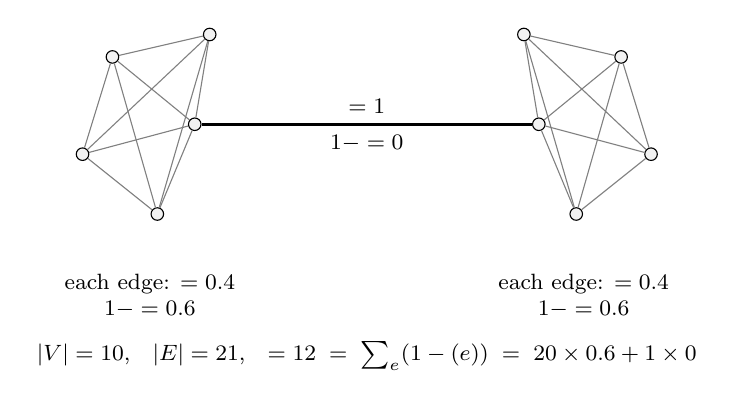
\begin{tikzpicture}[scale=0.95, every node/.style={font=\small}]
\definecolor{grey}{gray}{0.5}
% left cluster
\foreach \i/\x/\y in {0/0/0, 1/-1.1/0.9, 2/-1.5/-0.4, 3/-0.5/-1.2, 4/0.2/1.2} {
  \node[circle, draw, fill=black!5, inner sep=1.6pt] (a\i) at (\x,\y) {};
}
\foreach \i in {0,1,2,3,4} \foreach \j in {0,1,2,3,4}
  { \ifnum\i<\j \draw[grey] (a\i) -- (a\j); \fi }
% right cluster
\foreach \i/\x/\y in {0/4.6/0, 1/5.7/0.9, 2/6.1/-0.4, 3/5.1/-1.2, 4/4.4/1.2} {
  \node[circle, draw, fill=black!5, inner sep=1.6pt] (b\i) at (\x,\y) {};
}
\foreach \i in {0,1,2,3,4} \foreach \j in {0,1,2,3,4}
  { \ifnum\i<\j \draw[grey] (b\i) -- (b\j); \fi }
% bridge
\draw[very thick] (a0) -- node[above, font=\footnotesize]
  {$\Reff = 1$} node[below, font=\footnotesize] {$1-\Reff = 0$} (b0);
\node[font=\footnotesize, align=center] at (-0.6,-2.3)
  {each edge: $\Reff = 0.4$\\ $1-\Reff = 0.6$};
\node[font=\footnotesize, align=center] at (5.2,-2.3)
  {each edge: $\Reff = 0.4$\\ $1-\Reff = 0.6$};
\node[font=\footnotesize] at (2.3,-3.1)
  {$|V| = 10$, \; $|E| = 21$, \; $\bt = 12 \;=\; \sum_e (1-\Reff(e))
   \;=\; 20 \times 0.6 + 1 \times 0$};
\end{tikzpicture}}
\caption{The price code on a barbell engine graph. Twenty intra-cluster
engines each carry $0.6$ of detection strength; the bridge carries none.
The total is $\bt$ exactly (Theorem~\ref{eng:thm:foster}). A misquoted rate
inside a cluster produces a syndrome and is localisable; a misquoted rate
on the bridge is invisible.}
\label{eng:fig:barbell}
\end{figure}

\subsection{Decay along a pathway}\label{eng:S6.4}
\label{eng:sec:decay}

By \cite[Prop.~6.1]{vtok}, dissipation makes $\nu$ non-increasing along
engine operations. Along a path of length $d$ in the cost metric the
delivered value is $\nu e^{-\theta d}$. Set against the foraging
inequality's requirement that a harvest exceed the cost of obtaining it,
and taking a round-trip toll linear in $d$, a conversion at distance $d$ is
profitable iff $Y e^{-\theta d} > c\,d$.

\begin{proposition}[Profitable radius]\label{eng:prop:radius}
For $Y, c > 0$ and $\theta > 0$ the profitable set is an interval
$[0, d^\ast)$ with $d^\ast$ the unique root of $Y e^{-\theta d} = cd$.
There is a horizon on conversion set by metering, not by any speed limit.
\end{proposition}

Computed in Appendix~\ref{eng:app:repro} for $Y = 1000$, $c = 20$: $d^\ast =
19.17$ at $\theta = 0.05$, $8.73$ at $\theta = 0.2$, $1.52$ at $\theta =
\ln 10$, $0.82$ at $\theta = 5$.

\begin{remark}[The ecological pyramid is $\theta$]\label{eng:ecological-pyramid}
Predation is an engine: it converts prey-colour into predator-colour, and
it is spectacularly lossy. The classical figure of roughly ten per cent
transfer efficiency per trophic level \cite{lindeman} is
$r = 1/10$, i.e.\ $\theta = \ln 10 = 2.303$ per engine. The energy pyramid
is then exactly the exponential decay of $\nu$ along a path of engines,
which is Proposition~6.1 of \cite{vtok} with no adjustment. We did not
arrange this and record it as a check rather than a result.
\end{remark}

%% ===================================================================
\section{What conversion does to composition}\label{eng:S7}
\label{eng:sec:audit}

We audit the six results of \chComp under the addition of engines.

\paragraph{Factorisation survives and is sharpened.} An engine is a
spanning redex, so composed learners linked by one are dependent
(Proposition~\ref{eng:prop:convmet}). Two invariants of the same graph now
coexist: $\mathbf{k}$ counts edges of dependence, $\bt$ counts cycles of
it.

\paragraph{No metabolic mutualism needs qualification.} The proposition of
\S\ref{com:S6.1} of \chComp says that when overlap is confined to $\Met$ and
$\Src$, $\Delta_1 + \Delta_2 \leq 0$. Two things must be said.

\begin{proposition}[Dead stock]\label{eng:prop:nomet2}
Under (i) the total token supply of each colour is conserved by every
engine operation, and by \cite[Prop.~5.1]{vtok} the total $\nu$ is
conserved in the frictionless limit and strictly decreases under $\theta$.
So conversion is never positive-sum in value. But residual life is stack
divided by burn rate, and a token whose signature a learner cannot spend
contributes zero to its residual life and non-zero to the other's. Hence
conversion can strictly increase $\sum_i \sigma_i / b_i$ while conserving
$\nu$.
\end{proposition}

\begin{remark}[An honest gap in the source]\label{eng:honest-gap-source}
The proof sketch in \S\ref{com:S6.1} of \chComp argues that a transfer over a
shared metabolic name is ``strictly negative in aggregate residual life
whenever the two burn rates differ''. That step is directional: with
$\sum_i \sigma_i/b_i$ as the aggregate, a transfer toward the slower burner
raises it. In one colour the asymmetry is easy to miss because the
transfers that raise the aggregate are exactly the ones a predator has no
reason to make. Colours make it conspicuous, because dead stock is worth
zero to its holder by construction, so the profitable direction and the
aggregate-raising direction coincide. We therefore read the composition
note's proposition as correct about $\nu$ and in need of the qualification
above about residual life, and we take the qualification to be the content
of ``gains from trade'' in this setting.
\end{remark}

\begin{corollary}[The slogan, amended]\label{eng:slogan-amended}
\emph{Cooperation is epistemic; competition is metabolic} --- except where
the metabolisms are incommensurable, in which case conversion is
cooperative in residual life and still competitive in value. The
positive-sum region is exactly the region where signatures do not match.
\end{corollary}

\paragraph{Competitive dilution is re-coupled.} \S\ref{com:S9} of \chComp shows
that learners sharing a rate-limited source take shares $\propto 1/\text{cost}$
and that the dilution is regressive. Engines reinstate that competition
across boundaries that rooting had made clean: an engine is a shared name,
so conversion turns effective $k_{\mathrm{src}} = 0$ into effective
competition.

\begin{corollary}[Markets sell back modularity]\label{eng:markets-sell-back-modularity}
Rooting-by-quotation makes disjointness a theorem and thereby purchases
modularity; an engine sells it back at the price of the toll. Modularity
and tradability are opposed, and the grading vector prices the trade.
\end{corollary}

\paragraph{Phase, merger, succession.} Phase remains non-compositional.
Merger is now sharply distinguished from composition-with-engines: merger
identifies namespaces, an engine prices them, and \S\ref{eng:sec:indiv} says
when each is available. Succession --- a change of the grading vector
forced by source exhaustion --- acquires a second mechanism: an engine's
reserve running out changes $\Gamma$'s topology, and by
Theorem~\ref{eng:thm:foster} the code's total strength changes with it.

\begin{corollary}[Extinction degrades the price system]\label{eng:extinction-degrades-price-system}
Removing an engine from a cycle reduces $\bt$ by one and redistributes
$\Reff$; removing the last engine on a cut disconnects $\Gamma$ and
destroys the common numeraire. Loss of a converter is loss of
commensurability, not merely of throughput.
\end{corollary}

%% ===================================================================
\section{Individuation: where a namespace closes}\label{eng:S8}
\label{eng:sec:indiv}

\subsection{The three parameters, found inside the framework}\label{eng:S8.1}

\cite{compaut} locates the boundary between a shared substrate and
autonomous replication at a critical radius $r^\ast \sim
\sqrt{\rho v/\varepsilon}$. To transpose it we must find $\varepsilon$,
$\rho$, and $v$ inside the present framework rather than import them.

\begin{itemize}[itemsep=3pt]
\item $\varepsilon$, the \textbf{error rate}, is the per-hop drop-or-corrupt
rate $1-p$ of the interposed medium (\S\ref{eng:sec:medium}). This is the
channel \cite{compaut} is parameterised on --- error rate on transmission
--- and interposition supplies it natively rather than by analogy.
\item $\rho$, the \textbf{repair throughput}, is the rate of
retransmission, which by Corollary~\ref{eng:cor:owndepth} is available only
where the medium is nameable.
\item $v$, the \textbf{communication speed}, is $1/\theta$. There is no
speed in a cost-accounted calculus, but there is the temporal stack, and by
\cite[Prop.~4.1]{CE} time is the count of forced redexes. An expensive
pathway simply \emph{is} a slow one, and by
Proposition~\ref{eng:prop:twotheta} it is expensive for two reasons that enter
the same exponent.
\end{itemize}

Accidental name collision, which an earlier draft of this section took as
the error channel, is a second and different one: its failure mode is loss
of disjointness rather than loss of a message, and its repair is re-rooting
by freshness-by-quotation rather than retransmission. \S\ref{com:S7} of \chComp
proves it occurs. Hypothesis error is a third. \S\ref{eng:sec:whicheps}
returns to the question of which binds.

\begin{remark}[Why the medium channel is the one that individuates]\label{eng:why-medium-channel-one}
Collision threatens the \emph{identity} of names and is repaired by
re-quoting, which a region can do unilaterally. Loss threatens the
\emph{delivery} of messages and is repaired by retransmission, which a
region can do only over media it owns. Since Definition~\ref{eng:def:indiv}
turns on ownership of the internal medium, it is the transmission channel
that fixes the individuation threshold, and collision that fixes how
finely a namespace may be subdivided within it.
\end{remark}

\subsection{The structural form: partial closure}\label{eng:S8.2}

Proposition~\ref{eng:prop:indiv} below gives a quantitative threshold.
Definition~\ref{eng:def:indiv} gives a structural one --- the internal medium
is closed, the boundary medium is not --- and the two are the same
condition seen from two sides.

\begin{proposition}[Closure is what makes repair possible]
\label{eng:prop:closurerepair}
Retransmission over a medium $C$ requires grade-two access to $@C$, so
$\rho$ is supported only on $\Chn_{\mathrm{in}}(B)$. A region whose
internal media are not all nameable from within has $\rho$ effectively
reduced on the unnameable part, and by
Proposition~\ref{eng:prop:indiv} its sustainable radius falls accordingly.
\end{proposition}

\begin{corollary}[Bridges fail twice]\label{eng:bridges-fail-twice}
A boundary medium belongs to no region's closed internal namespace, so
neither party can unilaterally repair it. Together with
Theorem~\ref{eng:thm:detect} --- a bridge lies on no cycle and so carries no
syndrome --- a thin pathway is uncorrectable for two independent reasons:
nothing checks its rates, and nobody owns its medium.
\end{corollary}

\subsection{Isoperimetry replaces dimension}\label{eng:S8.3}

The derivation in \cite{compaut} balances errors accumulating over a volume
$r^d$ against repair delivered through a cross-section $r^{d-1}$, with a
propagation factor $v/r$. On a graph there is no dimension; the analogues
are the ball $B(r)$ and its edge boundary $\partial B(r)$, and their ratio
is the isoperimetric ratio $h(B) = |\partial B| / |B|$.

\begin{proposition}[Individuation threshold]\label{eng:prop:indiv}
A region $B$ of the engine graph may close over its namespace --- may be
merged, in the sense of \S\ref{com:S8} of \chComp --- iff repair keeps pace with
collision, that is iff
\[
  \rho\,|\partial B|\,\frac{1}{\theta\,r} \;\geq\; \varepsilon\,|B|,
  \qquad\text{equivalently}\qquad
  h(B) \;\geq\; \frac{\varepsilon\theta}{\rho}\, r .
\]
Writing $\kappa = \varepsilon\theta/\rho$, the individual is the largest
ball satisfying $h(B(r)) \geq \kappa r$.
\end{proposition}

\begin{corollary}[Recovering $r^\ast$]\label{eng:recovering-r}
On a graph of polynomial growth $d$ one has $h(B(r)) \sim c/r$, so the
condition becomes $c/r \geq \kappa r$ and
$r^\ast = \sqrt{c/\kappa} = \sqrt{c\rho/\varepsilon\theta}$, which is the
formula of \cite{compaut} with $v = 1/\theta$.
\end{corollary}

\subsection{Expansion}\label{eng:S8.4}

\begin{theorem}[Density buys exponentially larger individuals]
\label{eng:thm:expander}
If $\Gamma$ restricted to $B$ is an expander, $h(B(r)) \geq h_0 > 0$
uniformly, then $r^\ast = h_0/\kappa$ is linear rather than square-root in
$\rho/\varepsilon\theta$; and since an expander has diameter
$O(\log|B|)$, the merged population satisfies
$|B(r^\ast)| = e^{\Omega(r^\ast)}$. On a graph of polynomial growth $d$ the
merged population is only $|B(r^\ast)| = O((r^\ast)^d)$.
\end{theorem}

\begin{proof}
The first claim is Proposition~\ref{eng:prop:indiv} with $h$ bounded below.
The second is the standard fact that a family with $h \geq h_0$ has
diameter $O(h_0^{-1}\log n)$, so balls grow exponentially in radius.
\end{proof}

Theorem~\ref{eng:thm:expander} is the point at which the three threads of this
note become one. The ``densely connected component'' of the motivating
picture, the region where the price code is strong, and the region that may
close over its namespace are all the same region, and expansion is the
common criterion. Effective resistance is small exactly where expansion is
good; by Theorem~\ref{eng:thm:detect} detection is strong exactly where
effective resistance is small; and by Proposition~\ref{eng:prop:indiv} merger
is sustainable exactly where the boundary keeps up with the bulk.

Appendix~\ref{eng:app:repro}, block~(2), computes the merged population at four
values of $\kappa$ for a cycle, a $20\times 20$ grid, and random $3$- and
$6$-regular graphs on $400$ vertices. At $\kappa = 0.10$ the cycle sustains
an individual of $5$ colours, the grid $85$, the $3$-regular graph $160$,
and the $6$-regular graph $365$ --- the whole population.

\begin{figure}[t]
\centering
\fitwidth{%
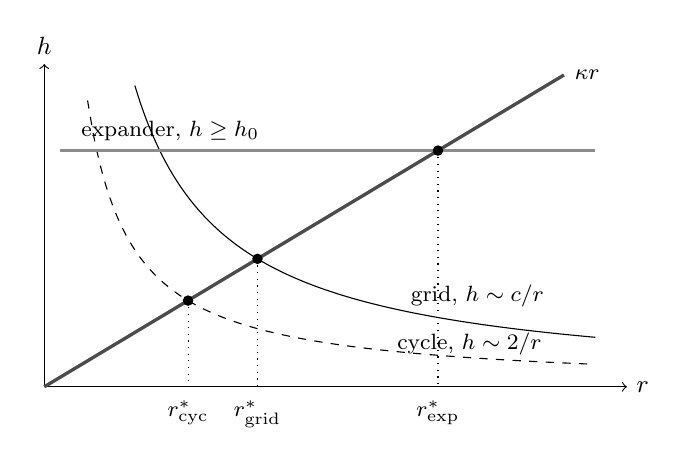
\begin{tikzpicture}[scale=1.0]
\draw[->] (0,0) -- (7.4,0) node[right, font=\small] {$r$};
\draw[->] (0,0) -- (0,4.1) node[above, font=\small] {$h$};
% kappa r line
\draw[very thick, black!70] (0,0) -- (6.6,3.96)
  node[right, font=\footnotesize, black] {$\kappa r$};
% cycle: h ~ 2/r
\draw[domain=0.55:7.0, samples=80, smooth, dashed] plot (\x, {2/\x});
\node[font=\footnotesize] at (5.4,0.55) {cycle, $h\sim 2/r$};
% grid: h ~ 4/r  (bigger constant)
\draw[domain=1.15:7.0, samples=80, smooth] plot (\x, {4.4/\x});
\node[font=\footnotesize] at (5.5,1.15) {grid, $h\sim c/r$};
% expander: constant
\draw[very thick, black!45] (0.2,3.0) -- (7.0,3.0);
\node[font=\footnotesize, black!45!black] at (1.6,3.25) {expander, $h\ge h_0$};
% crossings (computed: 2/x = .6x at x=1.826; 4.4/x = .6x at x=2.708;
%            3.0 = .6x at x=5.0)
\fill (1.826,1.095) circle (1.9pt);
\fill (2.708,1.625) circle (1.9pt);
\fill (5.0,3.0) circle (1.9pt);
\draw[dotted] (1.826,1.095) -- (1.826,0);
\draw[dotted] (2.708,1.625) -- (2.708,0);
\draw[dotted] (5.0,3.0) -- (5.0,0);
\node[font=\footnotesize, below] at (1.826,-0.05) {$r^\ast_{\mathrm{cyc}}$};
\node[font=\footnotesize, below] at (2.708,-0.05) {$r^\ast_{\mathrm{grid}}$};
\node[font=\footnotesize, below] at (5.0,-0.05) {$r^\ast_{\mathrm{exp}}$};
\end{tikzpicture}}
\caption{Individuation as a crossing. A region may be merged while its
isoperimetric ratio lies above the line $\kappa r$, $\kappa =
\varepsilon\theta/\rho$. Polynomially growing graphs cross early and give
$r^\ast \propto \kappa^{-1/2}$; an expander holds $h$ up and crosses late,
giving $r^\ast \propto \kappa^{-1}$ and, since balls grow exponentially in
$r$, an individual exponentially larger in population.}
\label{eng:fig:crossing}
\end{figure}

\subsection{What merger deletes}\label{eng:S8.5}

The intuition that centralisation buys compression and loses error
correction is right, and the framework can say precisely what is lost,
because merger destroys two different things.

\begin{proposition}[Merger sets $\bt = 0$]\label{eng:merger-sets-0}
A merged region has one colour, hence no engines internal to it, hence no
cycles in $\Gamma$ restricted to it. By Theorem~\ref{eng:thm:foster} its total
detection strength is zero. Centralisation does not degrade the price code;
it deletes it.
\end{proposition}

\begin{proposition}[Merger destroys independence]\label{eng:merger-destroys-independence}
By the factorisation theorem of \S\ref{com:S4.2} of \chComp, disjointness is
equivalent to $\mu_{12} = \mu_1 \otimes \mu_2$. Merger identifies
namespaces, so the joint distribution of a merged region does not factor
and failures are correlated.
\end{proposition}

These are detection and containment respectively, and they attach to
$\varepsilon$ and $\rho$ respectively. It is worth noting that the second
is exactly the third bullet of \cite[\S1]{compaut} --- the Fisher
information matrix is block-diagonal in the autonomous case and densely
off-diagonal in the shared case --- restated in the composition note's own
vocabulary. The two notes agreed before either knew it.

Against these, merger buys: no toll on internal transfers, since there are
no engines to pay; no arbitrage, since there are no cycles to carry it; and
the coordination compression of \cite[\S5]{vtok} in its limiting form,
where one does not even need the $n$ prices. That is the trade, priced on
both sides in one currency.

\subsection{Which $\varepsilon$ binds}\label{eng:S8.6}
\label{eng:sec:whicheps}

\cite{compaut} asks which error channel is rate-limiting in a cell and
conjectures proteostasis rather than genome integrity. We inherit the
question with three candidates, each with its own repair process and its
own throughput: \emph{transmission loss}, repaired by retransmission and
used above; \emph{name collision}, repaired by re-rooting; and
\emph{hypothesis error} --- the degrading prediction that the motivation
mechanism of \S\ref{sci:S2} of \chSci punishes --- repaired by revision. They
may well bind at different levels of the hierarchy, and the levels are
where the question becomes sharp: an organism's internal medium is
repairable and a pod's is not, so transmission should bind higher up and
collision lower down. The composition rule proposed in \cite{compaut},
$r^\ast = \min_i r^\ast_i$, applies; which $i$ attains the minimum at each
rung is open.

%% ===================================================================
\section{The hierarchy}\label{eng:S9}
\label{eng:sec:hier}

\subsection{Closure gives nesting; $r^\ast$ gives levels}\label{eng:S9.1}

Composition of learners yields a learner, so the construction is closed
under an associative operator and self-similarity costs nothing. But
closure permits arbitrary nesting; it does not select levels.

\begin{proposition}[Levels are forced by a finite $r^\ast$]\label{eng:levels-forced-finite-r}
If $r^\ast$ is finite, then a population exceeding $|B(r^\ast)|$ cannot be
maintained as one closed namespace, and the only way to continue scaling is
by replication of $r^\ast$-sized units composed with engines. Each
composite has its own effective $\varepsilon, \rho, \theta$, hence its own
$r^\ast$. The hierarchy is a sequence of critical radii.
\end{proposition}

The generating step is Proposition~\ref{eng:prop:tower}: the outside of one
level is the inside of the next. An orca's boundary media --- calls, touch,
the water --- are the pod's internal media, and the pod is an individual
exactly to the extent that it can name and repair them. So the tower of
media and the tower of individuals are the same tower, and neither has to
be posited alongside the other.

This is also the argument of \cite[\S6]{compaut} connecting $r^\ast$ to
West's allometry \cite{west}: the invariance of the terminal unit is a consequence
rather than a premise, and fractal replication above it is forced. Here the
same argument produces the levels the composition note could only permit.
The sequence terminates where $\theta \to \infty$ and even the cheapest
channel prices out.

\subsection{The shutoff ordering}\label{eng:S9.2}

Which components of $\mathbf{k}$ survive a given pathway cost? Price the
\emph{maintenance} of each type of overlap.

\begin{observation}[Ordering by maintenance cost]\label{eng:obs:order}
$\Met$ pooling requires continuous rendezvous and is the most expensive to
maintain. $\Mat$ requires periodic rendezvous. $\Src$ requires
co-availability at a rate-limited emitter. $\Prb$ requires only that a
legible surface stand where both can read it, and by the read-versus-drive
distinction of \S\ref{gam:S5.1} of \chGame a written surface costs nothing to leave
standing. Hence as $\theta$ rises the components extinguish in the order
$\Met$, $\Mat$, $\Src$, $\Prb$.
\end{observation}

\begin{table}[t]
\centering\small
\fitwidth{%
\begin{tabular}{@{}llll@{}}
\toprule
\textbf{Boundary} & \textbf{Operator} & \textbf{Surviving overlap}
& \textbf{Relation} \\
\midrule
within a skill set & $\Merge$ & all & one budget, one namespace \\
organism / organism & $\mid$ + engine & $\Met$ (transfer), $\Src$, $\Prb$, $\Mat$
& kin, trade, culture \\
deme / deme & $\mid$ + engine & $\Src$, $\Prb$, $\Mat$ & competition, culture \\
species / species & $\mid$ + engine & $\Src$, $\Prb$ & predation, eavesdropping \\
biosphere / biosphere & $\mid$ only & $\Prb$ & signals \\
beyond $d^\ast$ & --- & none & nothing \\
\bottomrule
\end{tabular}}
\caption{The hierarchy as a shutoff sequence. Each row is a level boundary,
identified by which component of the grading vector has gone to zero and
whether merger is still available. The ordering is
Observation~\ref{eng:obs:order}; the availability of $\Merge$ is
Proposition~\ref{eng:prop:indiv}.}
\label{eng:tab:levels}
\end{table}

\subsection{The grading vector is stratified, and has a fifth component}\label{eng:S9.3}

\begin{proposition}[A fifth typed namespace]\label{eng:prop:fifth}
$\Chn$ is a typed namespace in the sense of
\chComp, Definition~\ref{com:def:typed}, and overlap in it is not reducible to overlap in
the other four. Two learners sharing a medium can observe each other's
traffic and can congest each other, relations that
$\Met, \Src, \Prb, \Mat$ cannot express: eavesdropping, jamming, and
contention for bandwidth. Hence
\[
  \mathbf{k} \;=\; \bigl(k_{\mathrm{met}},\, k_{\mathrm{src}},\,
  k_{\mathrm{prb}},\, k_{\mathrm{mat}},\, k_{\mathrm{chn}}\bigr).
\]
\end{proposition}

\begin{remark}[This is very likely the arena]\label{eng:this-very-likely-arena}
\chComp leaves open whether the vector is complete and names the
\emph{arena} as the candidate fifth type; \chGame realises the arena
as the process routing moves between players. A router is a medium. We
therefore conjecture that the arena namespace and $\Chn$ are the same
namespace reached from two directions. We record this here rather than
amending \chComp, so that the two notes do not disagree in print
before that note is revised.
\end{remark}

\begin{corollary}[Composition and merger are the two halves of
$k_{\mathrm{chn}}$]\label{eng:composition-merger-two-halves}
Sharing a \emph{boundary} medium is composition: the learners talk,
interfere, and can trade. Sharing an \emph{internal} medium is merger, by
Definition~\ref{eng:def:indiv}. So the fifth component's in/out split is
exactly the distinction \S\ref{com:S8} of \chComp draws between its two
operators, which is evidence that the split is a refinement rather than an
epicycle.
\end{corollary}

\begin{corollary}[$\mathbf{k}$ is a sequence]\label{eng:k-sequence}
By Proposition~\ref{eng:prop:tower} the grading vector is relative to a
stratum, so the object that describes a composite fully is a sequence of
vectors, one per level of the medium tower. Table~\ref{eng:tab:levels} reads
off the sequence for one lineage.
\end{corollary}

Table~\ref{eng:tab:levels} has a pleasing consequence and a testable one. The
pleasing one: the last surviving channel is $\Prb$, which is exactly the
channel \chComp, Observation~\ref{com:obs:amort}, identifies as the only positive-sum one,
because formulae are not conserved. The testable one: the depth of the
hierarchy is the length of the grading vector, so the open question of
whether there is a fifth typed namespace --- the arena --- is the question
of whether there is a fifth level.

\subsection{An orca}\label{eng:S9.4}

An orca must solve hunting, position in the pod, mating, and care of young.
Suppose each is undergirded by a learner in the sense of \chComp.
Then:

The skills share one budget, so within the organism there is one colour, no
engines, and $\bt = 0$: \emph{there is no market inside an individual}. This
is Coase's theory of the firm \cite{coase} arriving unbidden.

Two claims must be kept apart here, and an earlier draft of this note ran
them together. That there is no \emph{market} inside an individual is a
claim about colour change: no rung-five medium, no conversion, allocation
by hierarchy rather than by price. That there is no \emph{mediation} inside
an individual would be a claim about the lower rungs of
Table~\ref{eng:tab:ladder}, and it is false --- an orca's internal
communication is as elaborate as anything it does, and by
Corollary~\ref{eng:cor:owndepth} that elaboration is precisely what closure of
the internal medium buys. Mediation is not allocation. The boundary of the
individual is where the token colour changes \emph{and} where the medium
stops being owned; the two coincide because an unowned medium cannot
sustain a shared budget.

The pod is not merged. Provisioning and food-sharing are transfers at
rates, hence composition with engines, and the framework predicts what is
observed: reciprocity with terms, not pooling.

Competitive dilution becomes a theory of skill acquisition. Skills at a
shared rate-limited source take shares $\propto 1/\text{cost}$, and the
regressive corollary of \S\ref{com:S9} of \chComp says dilution costs the
unfinished learner its depth and the finished one nothing. Inside one
organism this says a mature skill crowds out a developing one \emph{without
any contact between them}, which is automatisation and the critical period,
with a closed form.

And the instability of non-interference becomes development. Skills inside
one organism are rooted at the same quotation, so name coincidence is not
accidental but generic: the individual is precisely the regime in which the
disjointness theorem fails by construction. That is why skills interfere,
and why they transfer.

\begin{remark}[The orca claim is empirical, not definitional]\label{eng:orca-claim-empirical-definitional}
``Each skill is backed by a learner'' has content only if the skill
learners have distinct populations. If they are merely different formulae
held by one population, this is one learner with a large relaxation lattice
and the composition apparatus adds nothing. The discriminator is
\chSci, Proposition~\ref{sci:prop:confinement}: a single learner cannot leave its ball. So if
skills let each other escape basins, they must be separate populations, and
transfer between skills is the test.
\end{remark}

%% ===================================================================
\section{Incommensurability}\label{eng:S10}
\label{eng:sec:incomm}

Life elsewhere may not be organised around the same chemistry, and in this
framework that is not a matter of expense but of topology.

\begin{proposition}[No engine, no numeraire]\label{eng:no-engine-no-numeraire}
If no engine links the colours of two learners then $\Gamma$ is
disconnected, the connectedness hypothesis of \cite[Thm.~3.3]{vtok} fails,
and there is no common valuation: each component carries its own $\nu$ with
its own gauge. Incommensurability is disconnection.
\end{proposition}

\begin{theorem}[Commerce across an incommensurable boundary is epistemic]
\label{eng:thm:epistemic}
Let $\Lrn_1, \Lrn_2$ have disjoint $\Met$ and $\Src$ namespaces and no
engine between their colours. Then no token can pass between them. But by
\chComp, Observation~\ref{com:obs:two}, a formula is not conserved: a quotation $@P$
is inert while held, transmissible, and inspectable at grade three, and one
learner's coming to hold it does not deprive the other. Hence the only
available commerce is over $\Prb$.
\end{theorem}

Theorem~\ref{eng:thm:epistemic} is the slogan of \S\ref{com:S6} of \chComp scaled up
one level: between biospheres, cooperation is not merely the cheapest
positive-sum channel but the \emph{only} channel. Signals cross; food does
not. That is also consistent with Observation~\ref{eng:obs:order}, since $\Prb$
is the last component to extinguish, and the two arguments are
independent.

\begin{proposition}[First contact is a coincidence, not a construction]\label{eng:first-contact-coincidence-construction}
An engine requires a rendezvous, hence a shared name. Two ecologies rooted
at independent quotations are disjoint by
\S\ref{com:S7} of \chComp; but by the same section's remark, independently
manufactured names can coincide accidentally, and the exposure lemma of
\S\ref{sci:S9} of \chSci already records that closure is luck rather than
construction. So the establishment of a first engine between ecologies is a
structural coincidence whose probability is bounded by the name-growth
constraint of the no-self-code theorem.
\end{proposition}

We stop here. The obvious next question --- what a population of expanding,
converting ecologies does under these constraints, and whether
Proposition~\ref{eng:prop:radius}'s horizon reproduces or refutes the grabby
aliens hypothesis \cite{hanson} --- is left to \S\ref{eng:sec:open}.

%% ===================================================================
\section{Credit, default, and the discount rate}\label{eng:S11}
\label{eng:sec:credit}

The temporal combinators \texttt{truncate}$(t,c)$ and \texttt{get}$(c)$
denote claims on future value. In an ecology with a fixed $\Theta$ this
looks impossible: credit smells like minting. It is not.

\begin{proposition}[Credit is not minting]\label{eng:credit-minting}
A forward is a located slot whose release is gated on a temporal
condition. Nothing is created: the tokens exist and are held, and what
transfers is the right to receive on the slot. This is exactly the funding
slot of \cite[\S3.2]{finrho}, with the guard on the temporal stack rather
than on a signature.
\end{proposition}

\begin{proposition}[The discount rate is the hazard rate]\label{eng:discount-rate-hazard-rate}
A borrower that fails to repay in this setting is a starved borrower: by
\cite[Def.~1]{MC} and the metabolic law of \S\ref{sci:S5} of \chSci, failure
to fund is death. Credit risk is therefore mortality risk exactly, and the
rate at which a lender discounts a future claim is the borrower's hazard
rate, which the framework computes from stack over burn rate.
\end{proposition}

\begin{remark}[Options price the exploration budget]\label{eng:options-price-exploration-budget}
The choice combinators come with the conservative-bound discipline of
\cite[\S3.5]{finrho}: reserve the maximum over branches, refund the
unforced remainder. That is the exact structure of the question
\S\ref{sci:S6} of \chSci leaves open --- how much should a learner pay to keep
an unresolved hypothesis open? An option on a revision move has a premium,
a strike in metered units, and a refund on lapse, and the search-strategy
catalogue can be re-read as a portfolio problem. We flag this and do not
pursue it.
\end{remark}

%% ===================================================================
\section{On deriving the rates}\label{eng:S12}
\label{eng:sec:rates}

\cite{vtok} takes the rate function $r$ as given, and so has this note. It
should be derivable. The natural candidate is that the rate between two
colours is the ratio of marginal inquiry-yield per metered unit, which
\chGame computes exactly for its ladders: the non-modal rungs of the
noughts ladder deliver $+0.444$ of total gain for $87.9$ of $255.9$ units,
and the Nim ladders of \chComp give returns that are flat in one
environment and rising in another.

If that identification holds, then $\nu$ is a field over the ladder rather
than a bare price list, and the composition note's headline --- whether
truth is affordable is a property of the environment, not the learner ---
becomes a statement about exchange rates: communities working environments
where truth is cheap should systematically price their tokens differently
from communities where it is dear. This is checkable inside the existing
simulations and we regard it as the most tractable of the open problems.

%% ===================================================================
\section{What is shown, and what is not}\label{eng:S13}

Shown, in the sense of proved from the imported apparatus:
Theorems~\ref{eng:thm:detect}, \ref{eng:thm:foster} and \ref{eng:thm:expander};
Propositions~\ref{eng:prop:marking}, \ref{eng:prop:convmet}, \ref{eng:prop:series},
\ref{eng:prop:indiv}, \ref{eng:prop:radius}; and the merger propositions of
\S\ref{eng:sec:indiv}. These are graph theory and linear algebra over a
structure the earlier notes construct; they inherit whatever the earlier
notes' constructions are worth.

Shown by computation: the numbers of Appendix~\ref{eng:app:repro}, which are
exact where rational arithmetic was used and float otherwise.

Not shown: that the rates are what \S\ref{eng:sec:rates} conjectures; which of
the three error channels of \S\ref{eng:sec:whicheps} binds at which level;
that $\Chn$ is \chComp's arena, which is
conjectured and not proved; that the
identification of $v$ with $1/\theta$ is the only defensible one, as
opposed to the most natural; that inventory engines are the right reading
of the conservation fork, as against (ii); that the isoperimetric balance
in Proposition~\ref{eng:prop:indiv} has the right propagation factor, which is
inherited from \cite{compaut} and is heuristic there. The orca discussion
is illustration, not evidence, and \S\ref{eng:sec:hier} flags the test that
would make it evidence.

Not attempted: coherence of the lax monoidal structure of \chComp;
any dynamics on $\Gamma$ beyond the quasi-static drift of
Proposition~\ref{eng:prop:marking}; any treatment of strategic behaviour by
engines, which is where biological market theory \cite{noe} would enter.

%% ===================================================================
\section{Open problems}\label{eng:S14}
\label{eng:sec:open}

\begin{enumerate}[itemsep=4pt]
\item \textbf{Which $\varepsilon$ binds, and at which level.} Name
collision and hypothesis error are two channels with two repair processes.
Make $r^\ast = \min_i r^\ast_i$ precise and determine the minimising $i$ at
each rung of Table~\ref{eng:tab:levels}.
\item \textbf{Derive the rates.} Execute \S\ref{eng:sec:rates} against the
existing ladders and test whether exchange rates track environmental
structure as predicted.
\item \textbf{Dynamics on the engine graph.} Under (i) the marking drifts,
so $\bt$ is fixed but $\Reff$ moves and engines can die. Run the composite
of \S\ref{com:S10} of \chComp with engines under a Gillespie scheme and ask
whether the ecology self-organises toward an expander.
\item \textbf{Is $\Chn$ the arena?} Proposition~\ref{eng:prop:fifth} adds a
fifth typed namespace and conjectures it is \chComp's arena.
Settling this requires revising that note's relations table with a fifth
column and checking that the entries --- eavesdropping, jamming,
contention --- are not already derivable from the other four.
\item \textbf{Reordering.} Proposition~\ref{eng:prop:strand} covers dropping
and Table~\ref{eng:tab:ladder} covers corruption, but a medium may also
reorder, which is a race rather than a fault and which stranding does not
describe. Whether reordering is a third dissipation or a change in the
observed transition system is open.
\item \textbf{A syntactic criterion for porosity.}
Proposition~\ref{eng:prop:pathway} needs a decidable test that
over-approximates the existence of a redex pathway from a boundary
channel to an internal redex. Reuse the interaction graph of
\S\ref{sci:S12.5} of \chSci and measure the over-count.
\item \textbf{The assay trichotomy under loss.} A lossy medium introduces
a second source of the $\bot$ outcome that has nothing to do with budget,
and the learner cannot tell the two apart from inside. Budget-relative
refutation is therefore not well defined without a hypothesis about the
channel --- so a learner must do science on its own medium. This is a
correction owed to \S\ref{sci:S4} of \chSci rather than a problem for this
note, and we flag it here because this note is what raises it.
\item \textbf{Merger as a quotient, arbitrage-removal as a reflection.}
$\Merge$ identifies colours; $\Pi$ projects rates. Both take a conversion
structure to a simpler one, and \cite[\S4]{vtok} shows the second is an
idempotent reflection. Is there an adjunction relating them, with
Proposition~\ref{eng:prop:indiv} as the condition under which the left adjoint
exists?
\item \textbf{OSLF factoring and the crossover.} \cite{compaut} conjectures
that $r^\ast$ and the factoring of the generated logic over a population
are two views of one threshold. Proposition~\ref{eng:prop:indiv} gives the
first a graph-theoretic form; give the second one and compare.
\item \textbf{Grabby aliens.} With Proposition~\ref{eng:prop:radius}'s horizon,
Theorem~\ref{eng:thm:epistemic}'s restriction to signals, and the coincidence
bound on first contact, the expansion of a converting ecology is bounded by
profitability rather than by light speed. Whether that reproduces, softens,
or refutes the selection effects of \cite{hanson} is a question this
framework can now pose.
\end{enumerate}

%% ===================================================================

\section{Appendix: An engine, in rholang}\label{eng:S15}
\label{eng:app:rho}

The listing below gives located reserves, the reflexive observable, the
acceptance gate, the combinators, and the engine itself as a persistent
issuer offering a linear swap. Conventions follow \chGame: a parameter
written \texttt{c} is a name and \texttt{@d} is data; a channel is passed as
\texttt{*c}, since $@(*c) = c$; persistent receipts use \texttt{<=}.
Guards marked \texttt{//! ideal} use the \texttt{where} clause in a form the
current transpiler does not accept.

\begin{quote}
\small
\emph{Listing withheld from this printing.} The source of \texttt{engine.rho} was not committed alongside the other artefacts of this part and is not reproduced here; the construction it realises is given in full in \S\ref{eng:S4} and \S\ref{eng:S5} above.
\end{quote}

Three things to watch, tying the code to the propositions. The
\texttt{quote} face and the \texttt{swap} face are different names, because
perception must not be able to act --- grade one and grade two separated by
choice of namespace, as in \S\ref{gam:S4.1} of \chGame. The toll accrues to the
engine's own slot on every swap, which is Remark~\ref{eng:rem:eats}: $\theta$ is
not a parameter but a rendezvous. And \texttt{Observable} reads the
reserves and replaces them, which is Proposition~\ref{eng:prop:marking}: the
rate is a function of the marking, so the term itself refuses to let
arbitrage be a static property.

\section{Appendix: Reproducing the numbers}\label{eng:S16}
\label{eng:app:repro}

All figures in this note come from \texttt{engines.py}, four blocks.

\paragraph{(1) The price code.} Barbell of two $K_5$'s joined by one
engine: $|V| = 10$, $|E| = 21$, $\bt = 12$. An exact cochain has syndrome
$2.3 \times 10^{-15}$. Corrupting a single edge by $a = 1$ gives
$\|\ell_{\mathrm{arb}}\|^2 = 0.6$ for every intra-cluster edge
($\Reff = 0.4$) and $0$ for the bridge ($\Reff = 1$); the identity of
Theorem~\ref{eng:thm:detect} holds to $1.8\times10^{-15}$. The Foster identity
of Theorem~\ref{eng:thm:foster} is verified at $12.000000 = \bt$ for the
barbell, and separately for $K_5$ ($6$), $C_6$ ($1$), the $5\times5$ grid
($16$) and a random $3$-regular graph on $60$ vertices ($31$). Confusable
pairs: $0$ in the barbell, all $15$ in $C_6$. Mean detection strength for
random $d$-regular graphs on $60$ vertices: $0.344, 0.508, 0.672, 0.803,
0.902$ at $d = 3,4,6,10,20$, against the $1-2/d$ asymptote.

\paragraph{(2) Individuation.} Isoperimetric profiles for $C_{400}$, the
$20\times20$ grid, and random $3$- and $6$-regular graphs on $400$
vertices, and the largest ball satisfying $h(B(r)) \geq \kappa r$:

\begin{center}\small
\fitwidth{%
\begin{tabular}{@{}rrrrr@{}}
\toprule
$\kappa$ & $C_{400}$ & grid & $3$-regular & $6$-regular \\
\midrule
$0.30$ & $3$  & $25$  & $22$  & $151$ \\
$0.10$ & $5$  & $85$  & $160$ & $365$ \\
$0.03$ & $11$ & $219$ & $258$ & $365$ \\
$0.01$ & $19$ & $315$ & $349$ & $365$ \\
\bottomrule
\end{tabular}}
\end{center}

\paragraph{(3) Decay.} $Y = 1000$, $c = 20$, $d^\ast$ solving
$Ye^{-\theta d} = cd$: $19.172$ at $\theta = 0.05$; $8.728$ at $0.20$;
$1.518$ at $\ln 10$; $0.822$ at $5.0$.

\paragraph{(4) Inventory engines.} A triangle of constant-product engines,
each with reserves $(100,100)$, has cycle yield exactly $1$. Draining one
engine in steps of ten carries the yield through
\[
  0.827,\; 0.683,\; 0.562,\; 0.457,\; 0.367,
\]
that is, $\log \oint \ell$ from $0$ to $-1.0033$. Computed in exact
rationals.

\paragraph{(5) Porosity.} With $Y_0 = 100$, $Y(d) = Y_0(1-2^{-d})$,
$c = 2$, and net value $Y(d)p^d - cd$, the optimal integration depth and
its net value are:

\begin{center}\small
\fitwidth{%
\begin{tabular}{@{}rrrr@{}}
\toprule
$p$ & $d^\ast$ & net & $p^{d^\ast}$ \\
\midrule
$0.999$ & $5$ & $86.392$ & $0.9950$ \\
$0.990$ & $5$ & $82.127$ & $0.9510$ \\
$0.950$ & $3$ & $69.020$ & $0.8574$ \\
$0.900$ & $3$ & $57.788$ & $0.7290$ \\
$0.750$ & $2$ & $38.188$ & $0.5625$ \\
\bottomrule
\end{tabular}}
\end{center}

%% ===================================================================
